So far, only 2D monoblocks simulations were run, assuming an infinite thickness (or assuming no desorption from the poloidal gaps).
The goal of this section is to assess the influence of 3D edge effects on the monoblocks simulation results.
It will be shown that the error induced by 2D assumption decreases for thick monoblocks.

\subsection{Methodology}

The DEMO monoblock geometry differs slightly from the ITER geometry (see Figure \ref{fig: geometry DEMO monoblock}) but the general concept is the same, meaning the observations made in this Section are valid for the ITER geometry.


\begin{figure}
    \centering
        \begin{overpic}[width=\linewidth]{Figures/Chapter3/monoblocks/3D_monoblocks/sketch.pdf}
            \put(21, 15){\SI{23}{mm}}
            \put(51, 50){\SI{25}{mm}}
            % \put(21, 15){\SI{13.5}{mm}}
            \put(21, 56){ \diameter \SI{12}{mm}}
            \put(21, 63){ \diameter \SI{15}{mm}}
            \put(21, 68){ \diameter \SI{17}{mm}}
            \put(10, 70){\large$\Gamma_\mathrm{top}$}
            \put(0, 60){\large$\Gamma_\mathrm{lateral}$}
            \put(43, 60){\large$\Gamma_\mathrm{lateral}$}
            \put(21, 45){\large$\Gamma_\mathrm{coolant}$}
            \put(66, 71){\SI{4}{mm}}
            \put(66, 50){\SI{5}{mm}}
        \end{overpic}
    \caption{3D geometry of the DEMO monoblock used for the simulations.}
    \label{fig: geometry DEMO monoblock}
\end{figure}

The boundary conditions for the steady state heat transfer problem are the same as for the 2D case (see Equation \ref{eq: bc thermal DEMO monoblock}).
The boundary conditions for the transient H transport problem are similar (see Equations \ref{eq: bc H transport DEMO monoblock}).
A non-homogeneous mobile concentration is assumed at the plasma exposed surface to simulate an implanted source of particles (see Section \ref{triangle model}).
Depending on the simulation case (with or without desorption on the gaps), the other external surfaces (except the cooling surfaces) will either be insulated or an instantaneous recombination will be assumed.


\begin{subequations}
    \begin{align}
    -\lambda \vec{\nabla} T \cdot \vec{n} &=\varphi_\mathrm{heat} \quad  &\text { on } \Gamma_\mathrm{top}\\
    -\lambda \vec{\nabla} T\cdot \vec{n} &= -h \cdot \left(T_\mathrm{coolant} - T\right)\quad &\text { on } \Gamma_\mathrm{coolant}
    \end{align}
    \label{eq: bc thermal DEMO monoblock}
\end{subequations}
where $\varphi_\mathrm{heat}=\SI{10}{MW}$, $h=\SI{7e4}{W.m^{-2}.K^{-1}}$ is the heat exchange coefficient and $T_\mathrm{coolant} = \SI{323}{K}$ is the coolant temperature.

\begin{subequations}
    \begin{align}
    c_\mathrm{m} &=  \frac{\varphi_\mathrm{imp} R_p}{D} \quad &\text { on } \Gamma_\mathrm{top}\\
    -D \vec{\nabla} c_\mathrm{m} \cdot \vec{n} &= K_\mathrm{CuCrZr} \cdot c_\mathrm{m}^{2} \quad &\text { on } \Gamma_\mathrm{coolant} \\
    c_\mathrm{m} &=  0 \quad \text{or} \quad -D \vec{\nabla} c_\mathrm{m} \cdot \vec{n} = 0 &\text { on } \Gamma_\mathrm{lateral} \text{  and  } \Gamma_\mathrm{pipe}
    \end{align}
    \label{eq: bc H transport DEMO monoblock}
\end{subequations}
where $\varphi_\mathrm{imp} = \SI{1.6e22}{H.m^{-2}.s^{-1}}$ is the implanted particle flux, $R_p = \SI{1e-9}{m}$ is the particle implantation depth, $K_\mathrm{CuCrZr}=2.9\times 10^{-14}\exp{-1.92/(k_B T)}$ is the H recombination coefficient in CuCrZr expressed in \si{m^4.s^{-1}}.

Two intrinsic traps were set in W, one trap in the Cu interlayer and two traps in the CuCrZr cooling pipe (see Table \ref{tab:traps monoblock DEMO}).

\begin{table*}
    \centering
    \begin{tabular}{L{1.5cm} L{1.5cm} R{1.6cm} R{1.1cm} R{1.6cm} R{1.1cm} R{2cm}}
         & Material & $k_0 (\si{m^3.s^{-1}})$ &  $E_k (\si{eV})$ & $p_0 (\si{s^{-1}})$ & $E_p (\si{eV})$ & $n_i (\si{at.fr.})$ \\
        \hline
        \\
        Trap 1 & W & $9.0 \times 10^{-17}$ & 0.39 & $1 \times 10^{13}$& 0.78 & $1.0 \times 10^{-3}$ \\
        \\
       Trap 2 & W & $9.0 \times 10^{-17}$ & 0.39 & $1 \times 10^{13}$& 1.00 & $4.0 \times 10^{-4}$ \\
        \\
        Trap 3 & Cu & $6.0 \times 10^{-17}$ & 0.39 & $8.0 \times 10^{13}$ & 0.50 &$5.0 \times 10^{-5}$\\
        \\
        Trap 4 & CuCrZr & $1.2\times 10^{-16}$ & 0.42 & $8.0 \times 10^{13}$ & 0.50 &$5.0 \times 10^{-5}$\\
        \\
        Trap 5 & CuCrZr & $1.2\times 10^{-16}$ & 0.42 & $8.0 \times 10^{13}$ & 0.83 &$4.0 \times 10^{-2}$\\
        \\
    \end{tabular}
    \caption{Traps properties used in the 3D DEMO monoblocks simulations.}
    \label{tab:traps monoblock DEMO}
\end{table*}

Transient simulations up to \SI{e7}{s} were run.

\subsection{Standard case}

FESTIM simulations were run with and without desorption on the gaps.

% Temperature field

The temperature field obtained was very similar to the 2D case (see Figure \ref{fig: T field 3D monoblock}) with a top surface temperature of approximately \SI{1200}{K}.

\begin{figure} [h]
    \centering
    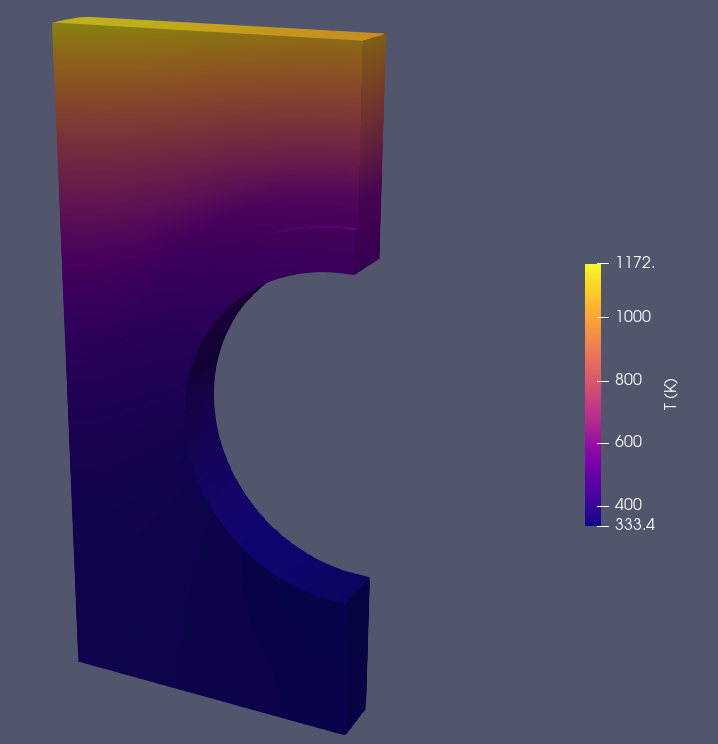
\includegraphics[width=\linewidth]{Figures/Chapter3/monoblocks/3D_monoblocks/temperature_3D_monoblock.png}
    \caption{Temperature field of the 3D DEMO monoblock.}
    \label{fig: T field 3D monoblock}
\end{figure}


% Retention fields
As expected, a higher retention was observed in the case without desorption (see Figure \ref{fig:retention fields 3D monoblocks}).
This is explained by the surface losses.
The maximum retention for the case with desorption is three orders of magnitude lower than that of the case without desorption.
In both cases, the higher retention was found to be in the CuCrZr cooling pipe.
This is consistent with the obsverations made previously.

\begin{figure} [h]
    \centering
    \begin{subfigure}{\linewidth}
        \centering
        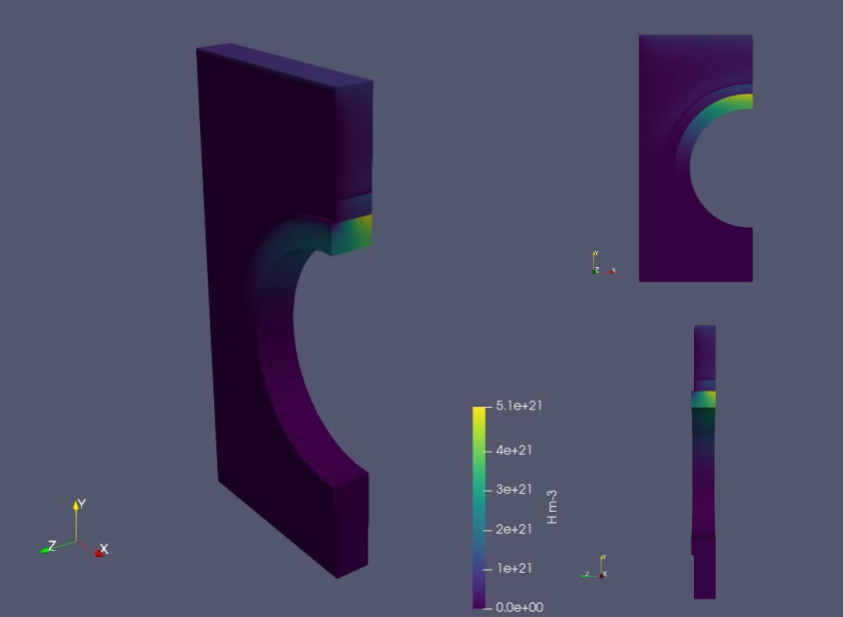
\includegraphics[width=\linewidth]{Figures/Chapter3/monoblocks/3D_monoblocks/MB 3D desorption.png}
        \caption{Instantaneous recombination on the gaps.}
    \end{subfigure}
    \begin{subfigure}{\linewidth}
        \centering
        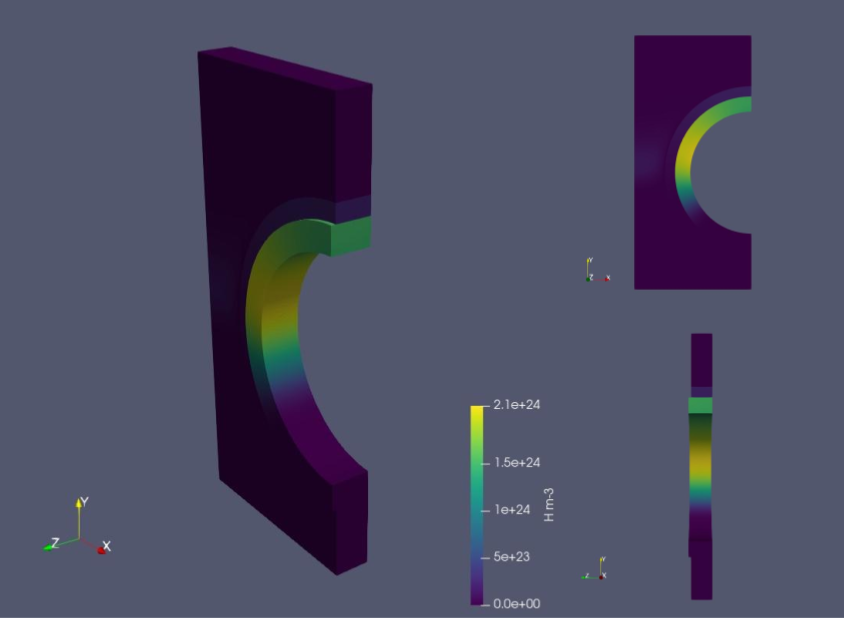
\includegraphics[width=\linewidth]{Figures/Chapter3/monoblocks/3D_monoblocks/MB 3D no desorption.png}
        \caption{No desorption on the gaps.}
    \end{subfigure}
    \caption{Retention fields of the DEMO monoblock after \SI{e7}{s} of continuous exposure with or without recombination on the gaps showing the isometric view (left), a central slice (top right) and a central clip showing the cooling pipe (bottom right). Note that the colour bars are different.}
    \label{fig:retention fields 3D monoblocks}
\end{figure}

% Inventory
The total H inventory in the monoblock was also between one and three orders of magnitude lower in the case with desorption (see Figure \ref{fig: inventory vs time DEMO monoblock}).
This difference increased with the exposure time.
Moreover, the steady state was reached way earlier for the case with desorption whereas the inventory kept increasing after \SI{e7}{s} for the insulated case.
This means that not taking desorption from the gaps into account in 2D simulations is a conservative assumption in terms of H inventory.
The simulations performed in Section \ref{influence of exposure conditions} then overestimate the monoblock H inventory.

\begin{figure} [h]
    \centering
    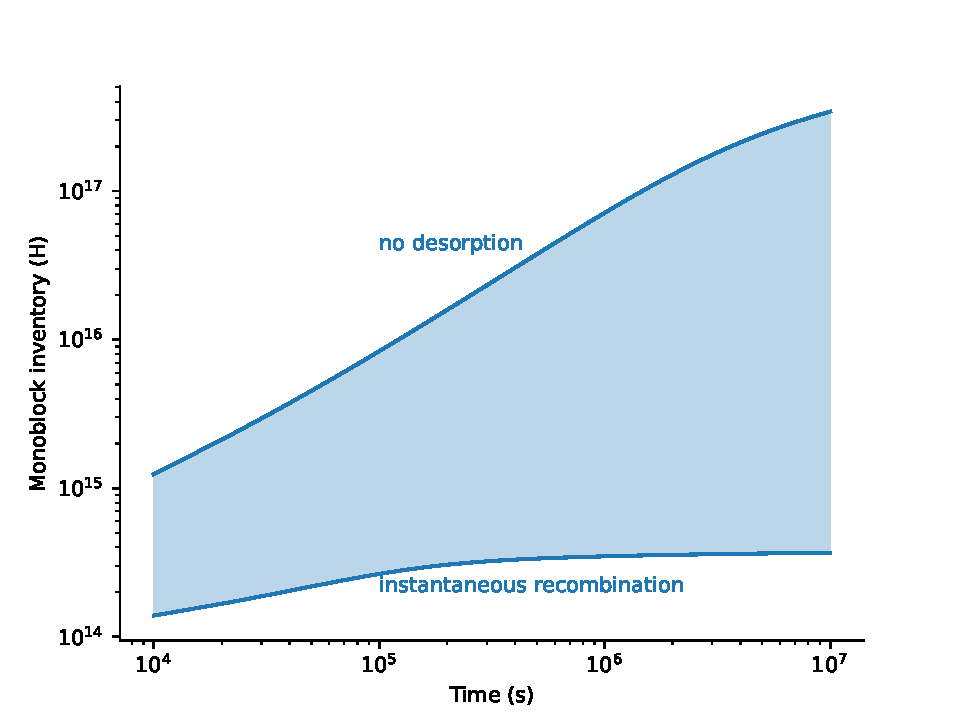
\includegraphics[width=\linewidth]{Figures/Chapter3/monoblocks/3D_monoblocks/inventory.pdf}
    \caption{Temporal evolution of the monoblock inventory.}
    \label{fig: inventory vs time DEMO monoblock}
\end{figure}

% fluxes
However, the outgassing fluxes from the monoblock gaps cannot be estimated with 2D (or 1D) simulations.
These fluxes were found to be five orders of magnitude higher than the permeation flux to the coolant: the particle flux towards the vacuum vessel was approximately \SI{e12}{H.s^{-1}} whereas the flux towards the cooling channel was below \SI{e8}{H.s^{-1}} (see Figure \ref{fig: fluxes DEMO monoblock}).
These fluxes can be compared to the retrodesorbed flux (\textit{ie} the flux of implanted particles that diffuse back to the exposed surface).
According to Equation \ref{eq:flux balance}, the value of this flux is equal to $\varphi_\mathrm{imp} \times \SI{23}{mm} \times \SI{4}{mm} = \SI{1.5e18}{H.s^{-1}}$.
The values of the outgassing fluxes from both the gaps and the cooling surface are therefore orders of magnitude lower than that of the retrodesorbed flux.
This means 3D edge effects will not affect previous results regarding the outgassing to the vessel.
They will however impact the value of the contamination flux towards the coolant as assuming an instantaneous recombination on the gaps will lead to way less particles reaching the cooling surface and therefore a lower flux.

\begin{figure} [h]
    \centering
    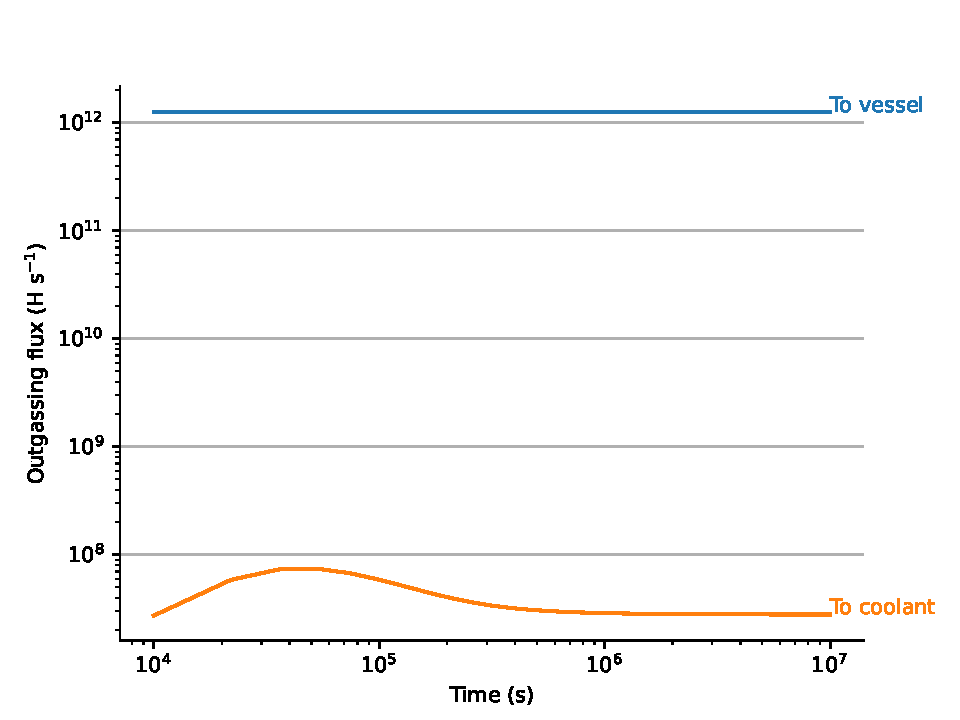
\includegraphics[width=\linewidth]{Figures/Chapter3/monoblocks/3D_monoblocks/fluxes.pdf}
    \caption{Temporal evolution of outgassing fluxes for the case with desorption from the gaps.}
    \label{fig: fluxes DEMO monoblock}
\end{figure}

\subsection{Influence of the monoblock thickness}

\begin{figure} [h]
    \centering
    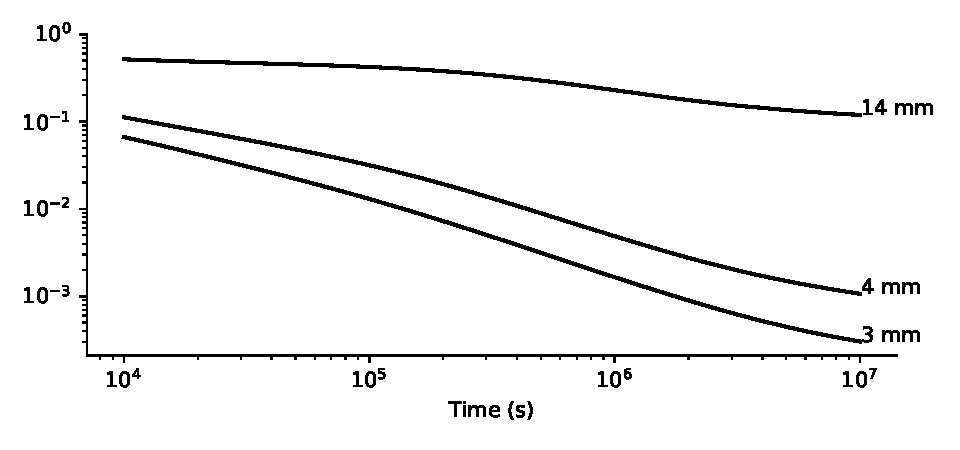
\includegraphics[width=\linewidth]{Figures/Chapter3/monoblocks/3D_monoblocks/influence_of_thickness.pdf}
    \caption{Temporal evolution of the ratio $\mathrm{inv}_\mathrm{desorption} / \mathrm{inv}_\mathrm{no desorption}$ for several thicknesses.}
\end{figure}

\subsection{Summary}